% -------------------------------------------------------------------
% Masterarbeit
% Kapitel 4: Implementierungstechniken
% Autor: Daniel Fritz
% Datum: 09.04.2016
% -------------------------------------------------------------------

\chapter{Implementierungstechniken}\label{chp:4:implementierungstechniken}
Dieses Kapitel stellt dar, aus welchen Teilen die Implementierung der Sprache aufgebaut ist. Ihre Funktion, ihre Implementierung und mögliche Alternativen werden gezeigt. Aufgrund des Inhalts dieser Arbeit beschränken sich Beispiele und Beschreibungen auch auf Java. Die Konzepte können jedoch auch auf andere Programmiersprachen übertragen werden. In den Abschnitten \ref{sct:4.1:eigenschaften} und \ref{sct:4.2:datenstrukturen} werden allgemeine Techniken vorgestellt, die oft bei der Implementierung einer Programmiersprache, insbesondere einer internen DSL verwendet werden. Die restlichen Abschnitte dieses Kapitels widmen sich den Implementierungen im Rahmen dieser Abschlussarbeit.

\section{Eigenschaften der Sprache}\label{sct:4.1:eigenschaften}
Der Bezug auf ein bestimmtes Arbeitsgebiet ist für eine Domänenspezifische Sprache obligatorisch. Zusätzlich zu dieser zwingenden Eigenschaft gibt es noch weitere Attribute, die häufig mit internen DSLs in Verbindung gebracht werden, auch wenn sie nicht zwingend erforderlich sind. Jedoch steigern sie die Lesbarkeit der Sprache und die Produktivität bei der Arbeit mit ihr. An dieser Stelle sollen diese Eigenschaften kurz beschrieben werden und beispielhaft erklärt werden, wie sie erreicht werden.

\subsection{Method Chaining}\label{ssct:4.1.1:chaining}
Method Chaining, das Aneinanderreihen von Methoden, wird von vielen direkt mit dem Aussehen einer internen DSL verbunden. Es ist zwar nicht zwingend notwendig, Method Chaining in einer internen DSL zu verwenden, jedoch ist es eine sehr nützliche Technik mit der der Sprachfluss und die Lesbarkeit einer Sprache deutlich verbessern kann \cite{book:fowlerDSL}. Ein kurzes Beispiel soll dies verdeutlichen.

Dafür nehmen wir an, dass eine Klasse \emph{Rezept} alle Zutaten für ein bestimmtes Rezept speichert. Da eine Vielzahl an Zutaten möglich ist, aber immer nur ein paar wenige für ein einzelnes Rezept nötig sind, werden sie der Klasse nicht per Konstruktor sondern per set-Methode übergeben. Normalerweise würde das folgendermaßen aussehen (alle Code-Beispiele sind in Java):\\

\begin{lstlisting}[caption=Erstellung eines Rezepts auf normale Weise]
	Recipe cake = new Recipe();
	cake.setButter(200);
	cake.setSugar(300);
	cake.setEggs(4);
	cake.setMilk(200);
	cake.setFlour(500);
\end{lstlisting}

\noindent
Dasselbe Rezept würde mithilfe von Method Chaining auf die folgende Weise zusammenstellt werden:\\


\begin{lstlisting}[caption=Erstellung desselben Rezepts mit Method Chaining]
	Recipe cake = new Recipe();
	cake.butter(200).sugar(300).eggs(4).milk(200).flour(500);
\end{lstlisting}

Um dieses Verhalten zu erreichen, müssen die einzelnen setter-Methoden anders als gewohnt implementiert werden. Üblicherweise würde eine Methode der Klasse so aussehen:\\

\begin{lstlisting}[caption=set-Methode in der üblichen Implementierung]
	public void setButter(int butterInGrams) {
		this.butter = butterInGrams;
	}
\end{lstlisting}

Um sie verketten zu können, müsste dieselbe Methode folgendermaßen implementiert werden:\\

\begin{lstlisting}[caption={set-Methode, implementiert zur Aneinaderreihung}]
	public Recipe butter(int butterInGrams) {
		this.butter = butterInGrams;
	}
\end{lstlisting}
\subsection{Method Nesting}\label{ssct:4.1.2:nesting}
Method Nesting beschreibt das Verschachteln von Funktionen, um hierarchische Strukturen abzubilden. Insbesondere wird dieses Vorgehen für rekursive Aufrufe genutzt \cite{book:fowlerDSL}, \cite{vl:drachen:teil3}. Letzteres wird erreicht, indem Rückgabewerte von Methoden als Argumente von Methoden einsetzbar sind.

In diesem Beispiel nehmen wir eine Sprache an, die Flächen beschreibt. Die Form der Fläche wird durch die Koordinaten einzelner Punkte angegeben. Der Code zeigt eine Fläche, die durch das Zusammensetzen zweier Flächen entsteht:

\begin{lstlisting}[caption=beispielhafte Verwendung von Method Nesting]
	Shape square = shape(point(0,0).point(0,1).point(1,1).point(1,0));
	Shape triangle = shape(point(0,1).point(0.5,2).point(1,1));
	
	Shape combine = shape(square.triangle);
\end{lstlisting}

\subsection{Object Scoping}\label{ssct:4.1.3:scoping}
Object Scoping erlaubt es, verkettete Methoden und die Zwischenergebnisse, welche bei der Verwendung auftreten, in einem Hostobjekt zu speichern. Die Alternative dazu ist das Speichern in globalen Variablen, was \glqq allgemein vermieden werden sollte\grqq~(übersetzt aus: \cite{book:fowlerDSL}).
\\ \\
Zusammen mit Method Chaining kann Object Scoping dazu verwendet werden, bestimmte Aufrufreihenfolgen innerhalb der Sprache festzulegen und so semantisch fehlerhafte oder unsinnige Eingaben bereits bei der Prüfung der statischen Syntax zu unterbinden. Diese Technik wird auch in dieser Abschlussarbeit verwendet (siehe auch Abschnitt \ref{ssct:4.3.2:treebuilder}).

\section{Datenstrukturen bei der Verarbeitung von Sprachen}\label{sct:4.2:datenstrukturen}
Jede Anweisung einer Sprache muss vom Computer \glqq verstanden\grqq~werden, bevor sie weiter verarbeitet werden kann. Nur in den einfachsten Fällen wird aus einer Eingabe direkt eine Ausgabe erzeugt. Ein Beispiel hierfür ist das Umwandeln eines Wiki-Markup-Formats in html \cite{book:parrLang}.
Damit ein Computer eine nicht-triviale Anweisung verstehen kann, muss er in Operatoren und Operanden zerlegt werden. Diese müssen in einer Datenstruktur abgelegt werden, die eine für die nachfolgenden Schritte geeignete Struktur aufweist. Zum einen ist wichtig, dass die Reihenfolge der einzelnen Elemente der Anweisung erhalten bleibt, zum anderen müssen die Beziehungen zwischen den Elementen abgebildet werden. Es hat sich herausgestellt, dass Bäume sich dafür am besten eignen \cite{book:parrLang}.

Generell kann hierbei zwischen zwei Arten von Bäumen unterschieden werden. Sie folgen logisch gesehen in der Verarbeitung hintereinander, müssen allerdings nicht immer beide verwendet werden.

Die eine Baum-Struktur ist der sogenannte Parse-Tree oder Syntax-Baum. Er besitzt eine Datenstruktur, in der sich speichern lässt, welche Regeln der Parser auf eine Anweisung angewendet hat und welche Terminalsymbole von ihm erkannt wurden \cite{book:parrLang}. Innere Knoten des Baums repräsentieren die Regeln, Blätter stehen für Terminalsymbole. Das Prinzip zur Erstellung von Parse-Trees ist einfach und regulär, daher können Syntaxbäume automatisch erstellt werden.\\
Die andere Baum-Struktur ist der abstrakte Syntax-Baum oder Abstract Syntax Tree (kurz: AST). Er repräsentiert, wie der Name vermuten lässt, die abstrakte Syntax-Struktur des Codes. Den AST zu einem Parse-Tree wird erstellt, indem aus dem Parse-Tree alle Knoten entfernt werden, die nur eine syntaktische und keine semantische Bedeutung haben \cite{book:parrLang}. Ein einfaches Beispiel für einen solchen Knoten ist das Semikolon am Ende einer Anweisung. Im AST bleiben nur Operatoren (innere Konten) und Operanden (Blätter).\\
Die folgende Abbildung verdeutlicht beispielhaft den Unterschied der beiden Baum-Typen anhand der Anweisung \texttt{x = 0;}:

\begin{figure}[H]
        \begin{subfigure}[b]{0.45\textwidth}
        	\centering
            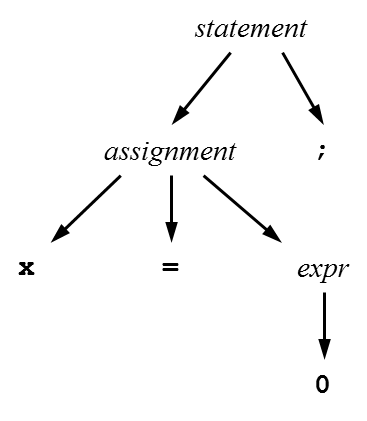
\includegraphics[width=\textwidth]{images/kapitel4/parseTreeGraph.png}
            \caption{Parse-Tree}
            \label{fig:bsp_disp_l}
        \end{subfigure}
        \begin{subfigure}[b]{0.30\textwidth}
            \centering
            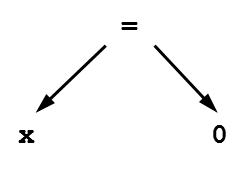
\includegraphics[width=\textwidth]{images/kapitel4/astGraph.png}
            \caption{AST}
            \label{fig:bsp_disp_r}
        \end{subfigure}
        \caption{Parse-Tree und AST der Anweisung \texttt{x = 0;}. Nachgezeichnet aus \cite{book:parrLang}.}
	    \label{fig:Beispiel_Disparitätsbild}
\end{figure}

Der große Vorteil des AST gegenüber dem Parse-Tree ist die Unabhängigkeit von der Syntax der Sprache. Das bedeutet, dass der AST und auch  nachfolgende Verarbeitungsschritte, die auf dem AST operieren, sich nicht ändern, wenn eine Umbenennung einer Regel in der Sprache vorgenommen wird. Außerdem kann der AST schneller als der Parse-Tree durchlaufen werden, weil die Anzahl der Knoten niedriger ist. Allerdings kann der abstrakte Syntax-Baum nicht vollautomatisch aus dem Parse-Tree generiert werden, sondern nur mithilfe von Regeln, die der Kenntnis der Sprach-Semantik bedürfen und diese widerspiegeln.

\section{Implementierung und verwendete Datenstrukturen}\label{sct:4.3:implementierung}
Die in Abschnitt \ref{sct:4.2:datenstrukturen} beschriebenen Datenstrukturen kommen - so oder in ähnlicher Form - im Rahmen dieser Abschlussarbeit vor. Ihre Implementierung und Verwendung werden in den folgenden Abschnitten detailliert beschrieben. Abbildung \ref{fig:komponenten} soll einen Überblick über die einzelnen Komponenten und ihr Zusammenspiel geben:

\begin{figure}[H]
\centering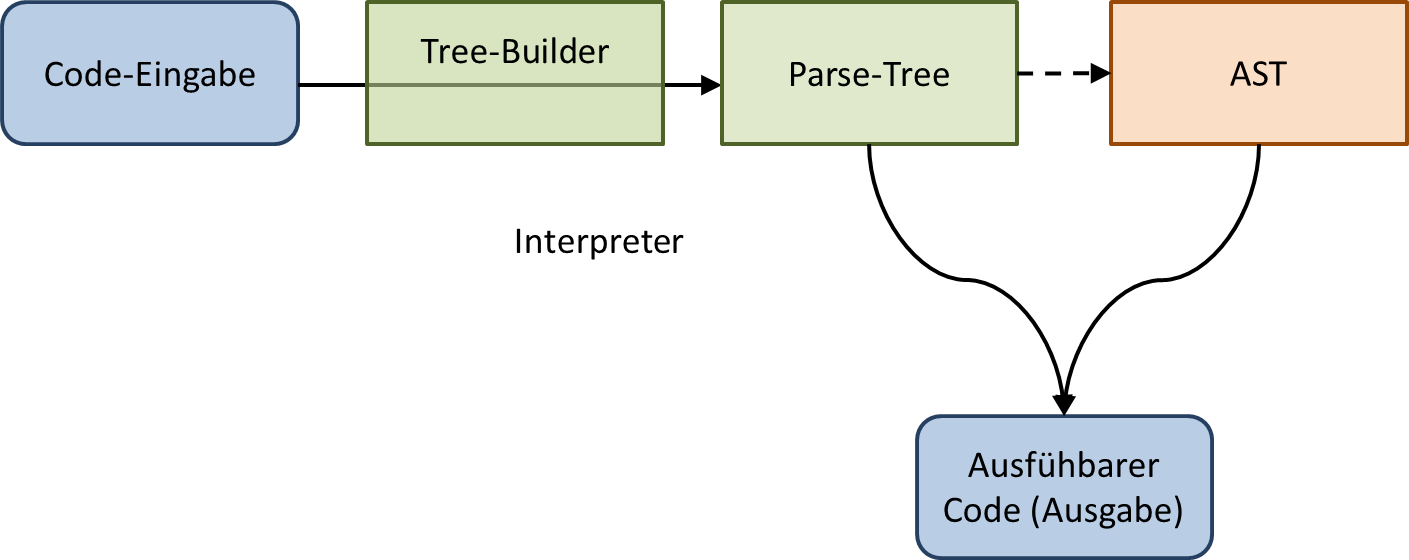
\includegraphics[width=.8\textwidth]{images/kapitel4/komponenten.png}
\caption{Komponenten der internen DSL}
\label{fig:komponenten}
\end{figure}

Die in Abschnitt \ref{sct:4.3:implementierung} beschriebenen Implementierungen sind ein Ergebnis dieser Abschlussarbeit. Sie werden in der Reihenfolge beschrieben, in der ein Sprach-Ausdruck verarbeitet wird. Abschnitt \ref{sct:4.4:alternativen} beschreibt alternativ mögliche Implementierungen.\\
Alle nachfolgend beschriebenen Codebeispiele der Implementierung beziehen sich auf eine DSL für arithmetische Ausdrücke, genannt \glqq Expression\grqq. Mit ihr lassen sich Rechnungen in den vier Grundrechenarten (\texttt{plus()}, \texttt{minus()}, \texttt{times()}, \texttt{divided}). Das erste Element eines Ausdrucks wird mit der Methode \texttt{expr()} gefasst, um eine Infix-Notation zu ermöglichen. Ihre Grammatik wird nachfolgend näher beschrieben.

\subsection{Definition einer Grammatik durch Interfaces}\label{ssct:4.3.1:grammatik}
Der erste Schritt bei der Implementierung einer Sprache ist das Festlegen der Grammatik. Sie beschreibt durch Regeln, wie ein Strom von Zeichen in einen Syntax-Baum umgewandelt wird \cite{book:fowlerDSL}. Die Grammatik soll, wie in \ref{sct:2.3:ziel} erwähnt, nur durch Interfaces festgelegt werden. Dabei soll es, wie in Abschnitt \ref{ssct:4.1.3:scoping} beschrieben, möglich sein, bestimmte Aufrufreihenfolgen festzulegen.

Eine in der EBNF formulierte Grammatik kann äquivalent als Flussdiagramm dargestellt werden. Anhand dieses Flussdiagramms können die dazugehörigen Interfaces folgendermaßen erstellt werden (übernommen und leicht abgeändert von \cite{www:jooq:fluentAPI}):

\begin{itemize}
	\item Jedes Schlüsselwort der DSL ergibt eine Java-Methode
	\item Jede Verbindung ergibt ein Interface
	\item Besteht die Wahl zwischen mehreren Schlüsselwörtern, ohne dass es die Möglichkeit gibt, diese zu überspringen, werden alle diese Schlüsselwörter Methoden in \emph{einem} Interface zusammengefasst.
	\item Gibt es ein Schlüsselwort, das wiederholt werden kann, dann hat die Methode, die aus diesem Schlüsselwort resultiert, als Rückgabewert den Typ ihres eigenes Interfaces und nicht den des nächsten.
	\item Kann das nächste Schlüsselwort optional ausgelassen werden, erweitert das aktuelle Interface das Interface mit jenem Schlüsselwort.
	\item Um Rekursion zu ermöglichen, haben betroffene Methoden den Objekt-Typ des Ergebnisses eines Ausdrucks als Parameter. \emph{Bemerkung:} Vollständige Unabhängigkeit zwischen einer Grammatik und ihrer Implementierung kann nur erreicht werden, wenn das Ergebnis eines Ausdrucks in der Sprach-Definition ein generischer Typ-Parameter ist. Bei der manuellen Implementierung wurde dies berücksichtigt. Aus zeitliche Gründen wurde bei der automatischen Generierung darauf verzichtet, da dies die Komplexität des Generators (siehe Kapitel \ref{chp:5:automatisierung}) erheblich erhöht. Stattdessen wurde der Typ \emph{ParseTree} (siehe auch Abschnitt \ref{sct:7.2:ausblick}) verwendet.
\end{itemize}

\begin{lstlisting}[caption={Grammatik der Expression-DSL, spezifiziert in EBNF},label=lst:grammar]
	Expression ::= expr '(' ([0-9]+ | Expression) ')'
	               (
	                    plus '(' ([0-9]+ | Expression) ')'
	                  | minus '(' ([0-9]+ | Expression) ')'
	                  | times '(' ([0-9]+ | Expression) ')'
	                  | divided '(' ([0-9]+ | Expression) ')'
	                )*
\end{lstlisting}

\begin{figure}[H]
\centering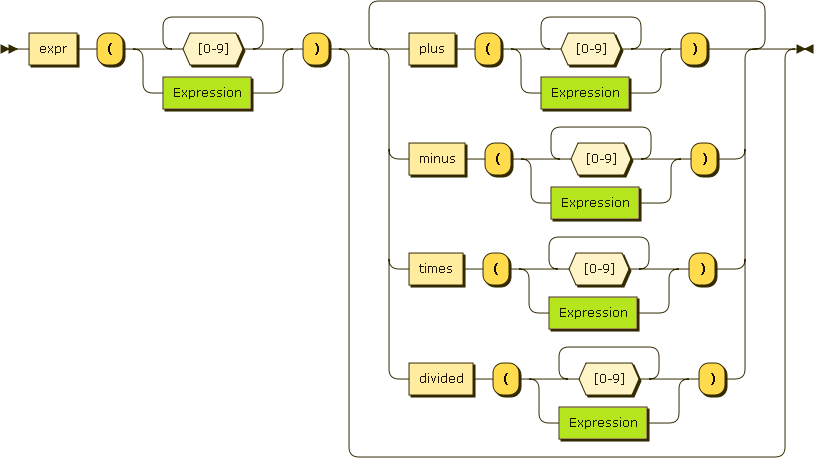
\includegraphics[width=.8\textwidth]{images/kapitel4/expressionRailroad.png}
\caption{Syntax-Diagramm der DSL. Grün eingefärbt: mögliche Rekursion.}
\label{fig:railroad}
\end{figure}

Beispiel-Code

\subsection{TreeBuilder und Scopes}\label{ssct:4.3.2:treebuilder}
Damit die Methoden der durch die Interfaces definierten Grammatik aufgerufen werden können, müssen die Interfaces implementiert werden. Mithilfe von Object Scoping (siehe Abschnitt \ref{ssct:4.1.3:scoping}) wird die gewünschte Aufrufreihenfolge der Methoden festgelegt. Dazu implementiert eine Klasse \textbf{\texttt{C}} jeweils die Methoden eines Interfaces \textbf{\texttt{I}}, inklusive der Methoden derjenigen Interfaces, die \textbf{\texttt{I}} erweitert. Der Inhalt der Methoden dient allein dem Aufbau der Parse-Tree-Struktur (siehe auch: Abschnitt \ref{ssct:4.3.3:parsetree}) und hat keinen semantischen Inhalt. Jede der genannten Klassen - im Folgenden auch speziell Scope-Klassen genannt - hat einen privaten Konstruktor. Dadurch wird verhindert, dass unkontrolliert ein Objekt dieser Klasse instantiiert wird, wodurch die Aufrufreihenfolge verletzt werden könnte.\\
Der Zugriff auf diese Klassen und deren Methoden erfolgt über eine Builder-Klasse, in die alle Scope-Klassen als innere Klassen eingebettet werden. Die Builder-Klasse hält eine private Instanz jeder Scope-Klasse, welche in ihrem Konstruktor erstellt wird. Jede Methode gibt entsprechend der festgelegten Aufrufreihenfolge das Scope-Objekt zurück, welches die nächste(n) erlaubte(n) Methode(n) enthält. Auch der Konstruktor der äußeren Klasse ist privat, da eine Instanz dieser Klasse für einen User keinen Nutzen hat - alle Felder und inneren Klassen sind privat. Stattdessen erfolgt der Zugriff über eine statische Methode (auch Einstiegsfunktion genannt; im Beispiel: \texttt{begin()}), welche gleichzeitig den Beginn eines jeden Ausdrucks der DSL markiert. Sie ruft den Konstruktor der äußeren Builder-Klasse sowie den derjenigen inneren Klasse auf, welche die erste Methode enthält. Sie gibt das zuletzt erstellte Objekt zurück. Danach kann die erste Methode der DSL aufgerufen werden, usw. Codeausschnitt \ref{lst:treebuilder1} zeigt beispielhaft den Code für eine Builder-Klasse.

\begin{lstlisting}[caption={Code für eine Builder-Klasse mit inneren Scope-Klassen},label=lst:treebuilder1]
	public final class TreeBuilder {
		private final OperatorScope operatorScope;
		
		// privater Konstruktor
		private ExprDSLTreeBuilder() {
			this.operatorScope = this.new OperatorScope();
		}
		
		// Einstiegs-Funktion
		public static StartScope begin() {
			return new ExprDSLTreeBuilder().new StartScope();
		}
		
		// Scope zum Interface "Start"
		public final class StartScope implements Start {
	
			private StartScope() {
			}
	
			@Override
			public OperatorScope expr(final double value) {
				// Code	
			}
			
			// ...
		}
		
		// Scope zum Interface "Operator"
		public final class OperatorScope implements Operator {
			// ...
		}
	}
\end{lstlisting}

Von der Scope-Klasse, welche die erste(n) Methode(n) eines Ausdrucks der DSL enthält, wird kein Objekt in der äußeren Klasse benötigt, da bereits die Einstiegsfunktion das entsprechende Objekt zurückgibt.

Die durch diese Implementierung erreichte Methoden-Verkettung in der DSL bringt den Nachteil des sogenannten \emph{finishing problem} \cite{book:fowlerDSL} mit sich. Es besagt, dass der Methoden-Kette ohne weitere Zusätze ein klarer End-Punkt fehlt. Ohne ihn bleibt ein Ausdruck immer unvollendet und kann nicht weiterverarbeitet werden. Es gibt mehrere Möglichkeiten, dieses Problem zu lösen. In der Implementierung dieser Abschlussarbeit wird eine abschließende Methode verwendet, die ein ParseTree-Objekt des entsprechenden Ausdrucks zurückliefert. Andere Möglichkeiten werden unter Abschnitt \ref{sct:4.4:alternativen} beschrieben. Diese Methode - hier \texttt{end()} genannt - wird in einem eigenen Interface platziert.\\
Die Implementierung dieser Methode sowie die vollständige Implementierung der TreeBuilder-Klasse werden im nächsten Abschnitt (\ref{ssct:4.3.3:parsetree}) im Zusammenhang mit der Syntax-Baum-Struktur erklärt.

\subsection{Parse-Tree}\label{ssct:4.3.3:parsetree}
Bei dieser Implementierung handelt sich um eine abgewandelte Form eines Syntax-Baums. Sie ist an DSLs angepasst, die in der Art entworfen wird, welche in dieser Abschlussarbeit vorgeschlagen werden. In der Datenstruktur des Parse-Tree werden, hierarchisch angeordnet, Scope- und Methoden-Knoten gespeichert, wobei ein Methoden-Knoten demjenigen Scope-Knoten zugeordnet ist, in dem die entsprechende Methode im TreeBuilder steht. Ein Parse-Tree-Objekt kann beliebig viele Scope-Knoten enthalten und ein Scope-Knoten beliebig viele Methoden-Knoten (sofern die Grammatik dies erlaubt). Abbildung \ref{fig:parse-tree} verdeutlicht den Aufbau der Datenstruktur:\\

\begin{figure}[H]
\centering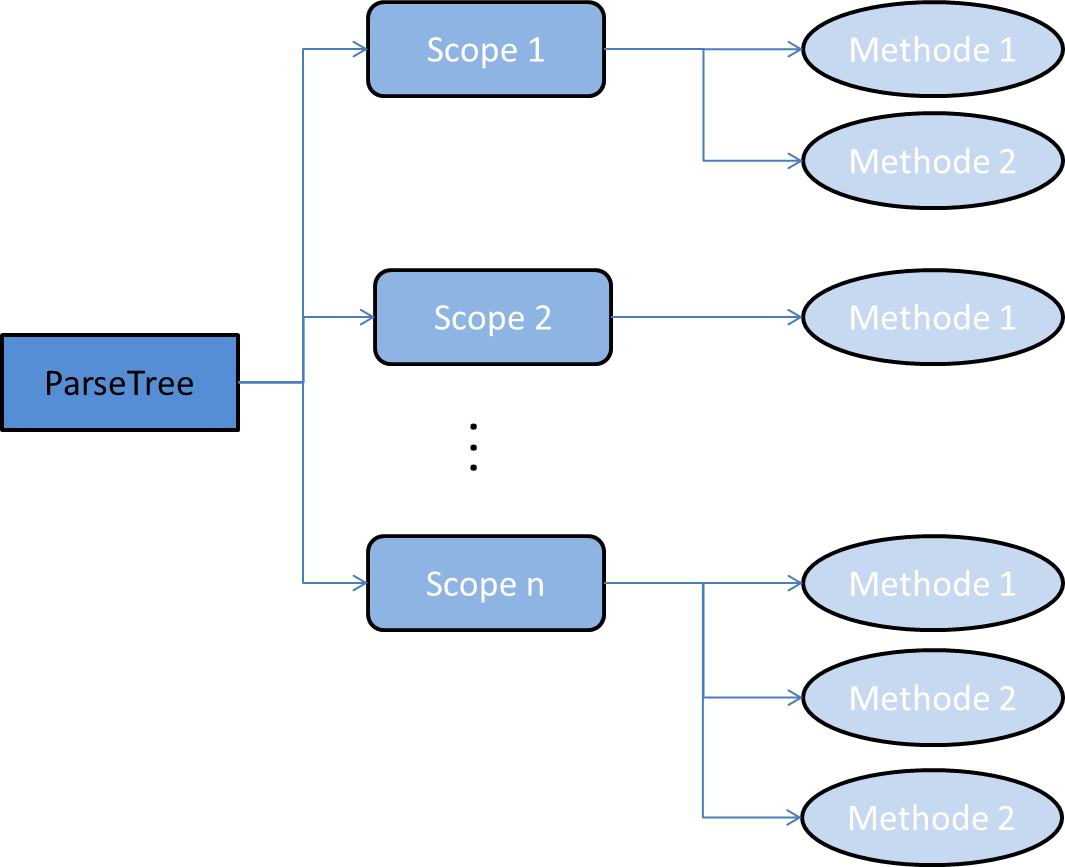
\includegraphics[width=.8\textwidth]{images/kapitel4/parseTree.png}
\caption{Komponenten der internen DSL}
\label{fig:parse-tree}
\end{figure}

Zu jeder Methode der DSL gibt es eine Methoden-Knoten-Klasse. Sie beinhaltet den Namen der Methode und den Wert des Parameters. Dazu hat sie einen Konstruktor, getter-Methoden für beide Felder und die überschriebene \texttt{toString()}-Methode. Um keinen überflüssigen Code schreiben zu müssen, werden Name der Methode und Wert des Parameters in zwei Stufen in abstrakte Oberklassen ausgelagert, welche von den konkreten Methoden-Knoten erweitert werden. Es wird grundsätzlich zwischen drei Methoden-Typen unterschieden: Diejenigen, die als Parameter \texttt{ParseTree} haben und damit Verschachtelung ermöglichen, alle anderen Methoden mit Parameter und Methoden ohne Parameter. Für die beiden Methoden-Typen mit Parameter gibt es eine eigene Oberklasse, die entweder ParseTree als Parameter oder einen generischen Typ-Parameter hat. Jede Methode kann höchstens einen Parameter haben. Dies erhöht in den meisten Fällen die Lesbarkeit der DSL und eliminiert gleichzeitig die Möglichkeit, Parameter einer Methode zu verwechseln. Methoden-Knoten ohne Parameter erben direkt von der obersten Methoden-Knoten-Klasse \texttt{AMethodNode}.\\
Analog zu den Methoden gibt es auch zu jeder Scope-Klasse eine ScopeNode-Klasse. Sie enthält den Namen des Scopes und eine Liste aller Methoden-Knoten, die entsprechend dem DSL-Ausdruck zu diesem Scope-Knoten gehören. Hier ist nur eine abstrakte Oberklasse - (\texttt{ASCopeNode} -  nötig, in der beide Felder und die dazugehörigen getter deklariert sind. \texttt{AScopeNode} implementiert das \texttt{Iterable}-Interface, um das Iterieren über \texttt{methods} mit einer for-each-Schleife zu ermöglichen.

\noindent
Abbildung \ref{fig:class-diagram1} in Abschnitt \ref{ssct:4.3.5:visitor} stellt den Zusammenhang zwischen den Klassen in einem UML-Klassendiagramm dar.

\subsection{Aufbau des Parse-Trees durch den TreeBuilder}\label{ssct:4.3.4:aufbau}
Die Konstruktion eines Parse-Tree-Objekts geschieht durch die Tree-Builder-Klasse: Wird eine Methode aufgerufen, erstellt sie einen Methoden-Knoten mit ihrem Namen und Parameter. Jede Scope-Klasse hat eine Liste, in der diese Methoden-Knoten in der Reihenfolge ihrer Erstellung abgelegt werden. Wird eine Methode aufgerufen, nach deren Aufruf der Scope gewechselt wird, dann wird mit der Methoden-Liste ein Scope-Objekt erstellt. Dieses wird wiederum in einer Liste in der äußeren Klasse gespeichert. Die abschließende Methode erstellt mit dieser Liste ein \texttt{ParseTree}-Objekt, welches sie zurückgibt. Auf diese Weise entsteht aus einem Ausdruck der DSL der dazu gehörige Syntax-Baum.\\
Listing \ref{lst:treebuilder2} zeigt für einzelne Methoden die vollständige Implementierung der TreeBuilder-Klasse.\\

\begin{lstlisting}[caption={vollständige Implementierung einer Builder-Klasse},label=lst:treebuilder2]
	public final class TreeBuilder {
		private ParseTree parseTree;
		private final OperatorScope operatorScope;
	
		private List<AScopeNode> scopes;
	
		private TreeBuilder() {
			this.operatorScope = this.new OperatorScope();
	
			this.scopeNodeList = new ArrayList<AScopeNode>();
		}
	
		public static StartScope begin() {
			return new TreeBuilder().new StartScope();
		}
		
		public final class StartScope implements Start {
			
			private List<AMethodNode> methodListStart;
	
			private StartScope() {
				methodListStart = new ArrayList<AMethodNode>();
			}
			
			@Override
			public Operator plus(final double value) {
				AMethodNode m = new SimpleMethodNodePlus(value);
				methodListOperator.add(m);
	
				return this;	
			}
	
			@Override
			public OperatorScope expr(final double value) {
				AMethodNode m = new SimpleMethodNodeExpr(value);
				methodListStart.add(m);
	
				// new ScopeNode
				AScopeNode scopeNodeStart = new ScopeNodeStart(methodListStart);
				TreeBuilder.this.scopeNodeList.add(scopeNodeStart);
	
				return TreeBuilder.this.operatorScope;	
			}
	
			// ...
		}
	
		public final class OperatorScope implements Operator {
	
			private List<AMethodNode> methodListOperator;
	
			private OperatorScope() {
				methodListOperator = new ArrayList<AMethodNode>();
			}
	
			@Override
			public Operator plus(final double value) {
				AMethodNode m = new SimpleMethodNodePlus(value);
				methodListOperator.add(m);
	
				return this;
			}
	
			@Override
			public ParseTree end() {
				AMethodNode m = new MethodNodeEnd();
				methodListOperator.add(m);
	
				// new ScopeNode
				AScopeNode scopeNodeOperator = new ScopeNodeOperator(methodListOperator);
				TreeBuilder.this.scopeNodeList.add(scopeNodeOperator);
	
				// new ParseTree
				parseTree = new ParseTree(scopeNodeList);
	
				return TreeBuilder.this.parseTree;	
			}
		}
	
	}
\end{lstlisting}

\subsection{Visitor}\label{ssct:4.3.5:visitor}
Beim nächsten Schritt in der Verarbeitung eines Sprach-Ausdrucks gibt es, wie in Abbildung \ref{fig:komponenten} bereits angedeutet, hauptsächlich zwei Möglichkeiten: Aus dem Syntaxbaum wird durch einen Interpreter direkt ausführbarer Code erzeugt oder ein von der Sprache unabhängiger abstrakter Syntaxbaum wird erstellt. Beide Varianten erfordern eine Möglichkeit, den Parse-Tree in Tiefensuche zu durchlaufen und bei jedem Knoten, wenn es die Semantik der Sprache erfordert, Code auszuführen.\\
In dieser Arbeit wurde dafür das in Sprachanwendungen häufig verwendete \cite{book:parrLang}, \cite{www:wiki:visitor} Besucher-Entwurfsmuster oder Visitor-Pattern der \emph{Gang of four} \cite{book:designPatterns} verwendet. Es erlaubt, Operationen in eine Objektstruktur zu integrieren, ohne diese bei jeder Änderung der Operationen anpassen zu müssen. Damit kann die Struktur des Syntax-Baums wie vorgesehen von seiner Auswertung getrennt werden.

Die Implementierung des Visitor-Patterns besteht aus folgenden Teilen:
\noindent
Das Interface \textbf{Visitable}, dessen Code im Listing \ref{lst:visitable} zu sehen ist, enthält nur die Methode \texttt{accept}. Dieses Interface wird von jedem Knoten des Parse-Trees, inklusive ParseTree selbst, implementiert. Bildlich gesprochen erlaubt der Knoten damit dem Visitor, ihn zu besuchen. Praktisch gesehen ruft er beim Visitor eine \texttt{visit}-Methode auf, welcher er als Parameter eine \texttt{this}-Referenz übergibt. Damit kann der Visitor auf die Eigenschaften des Knotens zugreifen.\\

\begin{lstlisting}[caption={Code des Visitable-Interfaces},label=lst:visitable]
	public interface Visitable {
		void accept(AVisitor visitor);
	}
\end{lstlisting}

Der \textbf{Visitor} selbst ist eine einzelne Klasse. Sie besitzt für jede Knoten-Klasse des Syntax-Baums eine \texttt{visit}-Methode, in der definiert ist, welcher Code beim Besuch dieses Knotens auszuführen ist. Dadurch, dass jede Knoten-Klasse direkt \texttt{accept()} implementiert, wird der Aufruf an die richtige \texttt{visit()}-Methode weitergeleitet.\\
Um Coderedundanz zu vermeiden, gibt es für alle konkreten Visitor-\\Implementierungen eine abstrakte Oberklasse \texttt{AVisitor}, welche bereits den Besuch des ParseTree-Objekts implementiert.\\

Damit ergibt sich für die Knoten-Klassen folgendes Klassen-Diagramm:

\begin{figure}[H]
\centering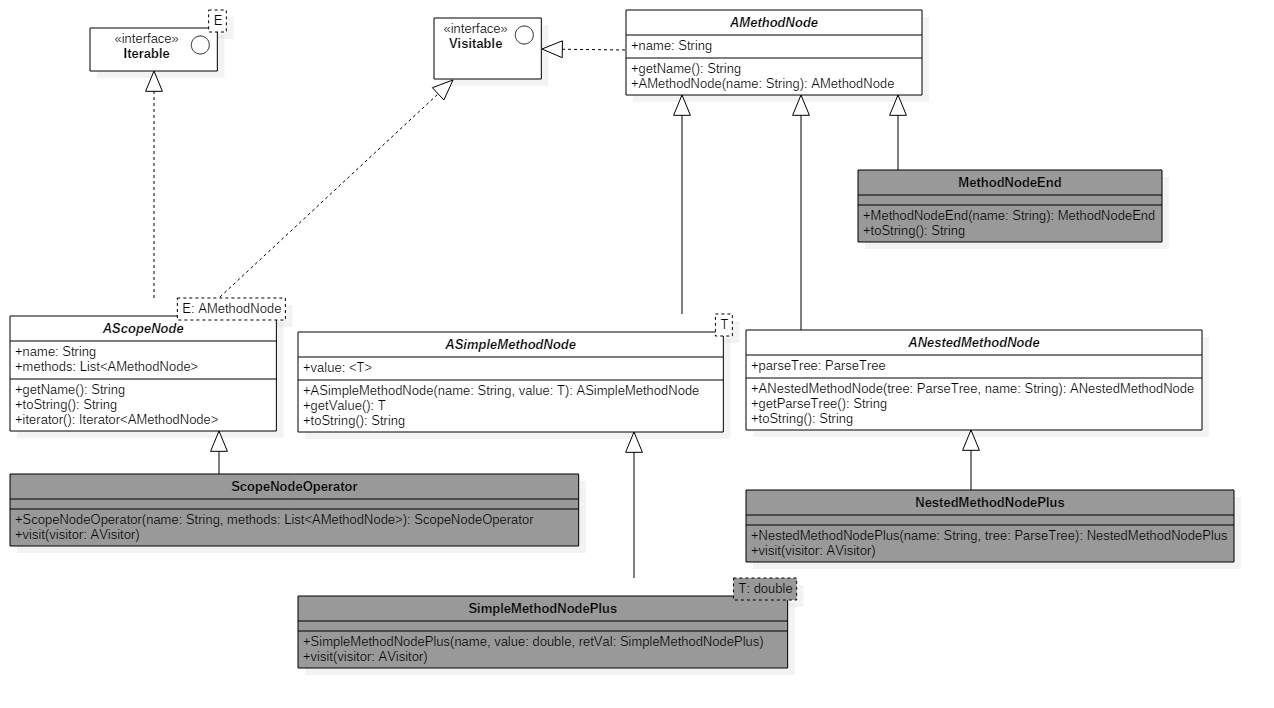
\includegraphics[width=1.1\textwidth]{images/kapitel4/classDiagram1.png}
\caption{Klassendiagramm aller Knoten-Klassen des Syntax-Baums. Grau eingefärbt sind beispielhafte konkrete Knoten-Klassen.}
\label{fig:class-diagram1}
\end{figure}

Der Visitor implementiert das sogenannte \emph{double dispatch}, da die ausgeführte Operation sowohl vom Typ des Visitors als auch von dem Element, welches besucht wird, abhängt \cite{www:visitor-sourcemaking}.
%Danach:
%AST erwähnen
%nochmal erklären, warum Aufteilung in Grammatik, TreeBuilder, ParseTree (und AST) Vorteile mit sich bringt.
%Note, it is possible to model the above DSL with classes instead of interfaces, as well. But as soon as
%you want to reuse similar keywords, multiple inheritance of methods may come in very handy and
%you might just be better off with interfaces.

\section{Alternative Implementierungen}\label{sct:4.4:alternativen}
Für die in Abschnitt \ref{sct:4.2:datenstrukturen} beschriebenen Datenstrukturen sind alternative Implementierungen möglich, welche in diesem Abschnitt erläutert werden sollen.

Grundsätzlich ist es möglich, den Zwischenschritt des Syntax-Baums wegzulassen. Stattdessen baut man direkt im TreeBuilder den AST auf. Dies kann bei kleinen Sprachen die Entwicklung vereinfachen, macht die Implementierung aber schnell unübersichtlich und schwer zu ändern.
jedoch separation of concerns verletzten, die in dieser Arbeit bewusst gewollt und gefordert war.

\subsection{TreeBuilder und ParseTree}\label{ssct:4.4.1:alt-treebuilder-parsetree}
Anstatt das \emph{ParseTree}-Objekt am Ende einer Aufruf-Kette zu erstellen, könnte dies schon im Konstruktor des Tree-Builders geschehen. Ein Knoten-Objekt wird direkt nach der Erstellung an den ParseTree gereicht, der es entsprechend einfügt. Der Nachteil gegenüber der vorgenommenen Implementierung ist hierbei, dass zusätzliche Methoden benötigt werden, um die Baum-Knoten innerhalb des ParseTree an der richtigen Stelle zu platzieren.

\subsection{Baum-Knoten und Visitor}\label{ssct:4.4.2:alt-knoten-visitor}
Statt für jede Methode und jeden Scope eine Baumknoten-Klasse zu haben, gibt es die alternative Möglichkeit, nur drei verschiedene Klassen zu verwenden. Dazu werden die abstrakten Klassen \texttt{ASimpleMethodNode} und \texttt{ANestedMethodNode} (siehe Abschnitt \ref{ssct:4.3.3:parsetree} und Abbildung \ref{fig:class-diagram1}) als konkrete Klassen verwendet. Analog dazu gibt es auch nur eine ScopeNode-Klasse. Der Vorteil daran ist, dass die Implementierung der Sprache weniger Klassen hat; bei einer größeren Sprache kann das ein beträchtlicher Unterschied sein. Der Nachteil ist, dass im Visitor für jeden Scope- und Methodenknoten der Name abgefragt werden muss, um den passenden Code auszuführen. Dies wird bei größeren Sprachen schnell unübersichtlich.